
%Use only LaTeX2e, calling the article.cls class and 12-point type.
%Tandy is editing on March 6
\documentclass[12pt]{article}
%
%Users of the {thebibliography} environment or BibTeX should use the
%scicite.sty pack$output_dir/upp_results/upp_$query_size\_$align_size\_mafft_L-INS-i_alignment_masked $output_dir/upp_results/upp_$query_size\_$align_size\_mafft_L-INS-i_alignment_masked age, downloadable from *Science* at
%www.sciencemag.org/about/authors/prep/TeX_help/ .
%This package should properly format in-text
%reference calls and reference-list numbers.  
%
\usepackage{amsmath}
\usepackage{graphicx}
\usepackage{bigstrut}
\usepackage{color}
\usepackage{multirow}
\usepackage{hhline}
\usepackage{graphics}
\usepackage{hyperref}
\usepackage[export]{adjustbox}
\usepackage{listings}
\usepackage{float}
\usepackage{subfig}
%
%Use times if you have the font installed; otherwise, comment out the
%following line.
%
\usepackage{times}

% The preamble here sets up a lot of new/revised commands and
% environments.  It's annoying, but please do *not* try to strip these
% out into a separate .sty file (which could lead to the loss of some
% information when we convert the file to other formats).  Instead, keep
% them in the preamble of your main LaTeX source file.

% The following parameters seem to provide a reasonable page setup.
%\DeclareGraphicsRule{.tif}{png}{.png}{`convert #1 `dirname #1`/`basename #1 .tif`.png}
\topmargin 0.0cm
\oddsidemargin 0.2cm
\textwidth 16cm 
\textheight 21cm
\footskip 1.0cm


\renewcommand\refname{References and Notes}

% The following lines set up an environment for the last note in the
% reference list, which commonly includes acknowledgments of funding,
% help, etc.  It's intended for users of BibTeX or the {thebibliography}
% environment.  Users who are hand-coding their references at the end
% using a list environment such as {enumerate} can simply add another
% item at the end, and it will be numbered automatically.

\newcounter{lastnote}
\newenvironment{scilastnote}{%
\setcounter{lastnote}{\value{enumiv}}%
\addtocounter{lastnote}{+1}%
\setcounter{page}{1}
\begin{list}%
{\arabic{lastnote}.}
{\setlength{\leftmargin}{.22in}}
{\setlength{\labelsep}{.5em}}}
{\end{list}}


% Include your paper's title here

%\title{ViFi Supplemental Material} 
%
%\author
%{Nam-phuong Nguyen$^{1}$, Viraj Deshpande$^{1}$, 
%Jens Luebeck$^{2}$, Paul S. Mischel$^{3,4,5}$, and Vineet Bafna$^{1}$\\
%\normalsize{$^{1}$Computer Science and Engineering, University of California,}\\
%\normalsize{San Diego, La Jolla, 92093, USA.,}\\
%\normalsize{$^{2}$Bioinformatics and Systems Biology Program, University of California,}\\
%\normalsize{San Diego, La Jolla, 92093, USA.,}\\
%\normalsize{$^{3}$Ludwig Institute for Cancer Research, University of California,}\\
%\normalsize{San Diego, La Jolla, 92093, USA.,}\\
%\normalsize{$^{4}$Department of Pathology, University of California,}\\
%\normalsize{San Diego, La Jolla, 92093, USA.,}\\
%\normalsize{$^{5}$Moores Cancer Center, University of California,}\\
%\normalsize{San Diego, La Jolla, 92093, USA.}\\
%\normalsize{$^\ast$To whom correspondence should be addressed; E-mail:  vbafna@eng.ucsd.edu.}
%}

\begin{document}
\section*{Online supplemental materials}
\setcounter{figure}{0}
\renewcommand{\thesection}{S\arabic{section}}   
\renewcommand{\thefigure}{S\arabic{figure}}   
\renewcommand{\thetable}{S\arabic{table}}   
\section{ViralFusionSeq debugging}\label{vfs_error}
During the process of running ViralFusionSeq~\cite{Li2013}, we discovered several bugs in the code that had
to be fixed in order for ViralFusionSeq to have the proper behavior.  These bugs were confirmed
during an email discussion with the ViralFusionSeq authors about running the software.  Even
with the changes, we were unable to complete running ViralFusionSeq on any datasets.  These difficulties lead us to exclude ViralFusionSeq in our analyses.

\section{Running ViralFusionSeq}\label{vfs_commands}
ViralFusionSeq takes as input a configuration file, an output name, and the input FASTQ files.  

\paragraph{\textbf{ViralFusionSeq (version 2.0)}}
\begin{itemize}
\item{\textbf{Running ViralFusionSeq}} \emph{perl viral.fusion.pl --config $<$configuration\_file$>$ $<$output\_name$>$ $<$input\_fastq\_1$>$ $<$input\_fastq\_2$>$}
\end{itemize}

The configuration file contains the paths to software tools used within ViralFusionSeq and the paths to the human and viral reference databases.  The ViralFusionSeq configuration file is available on the ViFi GitHub page.

\section{VERSE error message}\label{verse_error}
VERSE~\cite{Wang2015} would fail to complete due to two conditions.  First, is if VERSE took longer than 48 hours to run, and second, if VERSE terminated early without outputting an integration file.  Below is a common error message that
is outputted during a failed run.  
\begin{lstlisting}[basicstyle=\footnotesize]
Use of uninitialized value \$temp[1] in addition (+) atVirusFinder.pl line 584 
    (#1) (W uninitialized) An undefined value was used as if it were already
    defined.  It was interpreted as a "" or a 0, but maybe it was a mistake.
    To suppress this warning assign a defined value to your variables.

    To help you figure out what was undefined, perl will try to tell you the
    name of the variable (if any) that was undefined. In some cases it cannot
    do this, so it also tells you what operation you used the undefined value
    in.  Note, however, that perl optimizes your program and the operation
    displayed in the warning may not necessarily appear literally in your
    program.  For example, "that \$foo" is usually optimized into "that "
    . \$foo, and the warning will refer to the concatenation (.) operator,
    even though there is no . in your program.

Uncaught exception from user code:
        Use of uninitialized value \$temp[1] in addition (+) at VirusFinder.pl 
        line 584. at VirusFinder.pl line 584
        main::RunSensitiveMode() called at VirusFinder.pl line 282
        main::DetectIntegration() called at VirusFinder.pl line 214
}
\end{lstlisting}


\section{VERSE optimization}\label{verse_opt}
In order to have VERSE run more efficiently, we changed VERSE's default behavior of outputting uncompressed SAM file directly to disk before converting to a compressed BAM file to piping the SAM file directly into a compressed BAM file.  This resulted in a four-fold reduction in disk space usage running each run.

Thus, these pair of lines,

\begin{lstlisting}[basicstyle=\footnotesize]
    `$bowtie_bin -p $thread_no -D 15 -R 2 -N 0 -L 22 -i S,1,1.15 -x 
    $bowtie_index_human -1 $fastq1 -2 $fastq2 -S $output_dir/alignment.sam`;
    print "Convert SAM alignment file to BAM file...\n";
    `samtools view -bS $output_dir/alignment.sam -o $alignment_file`;
\end{lstlisting}
    
were changed into a single line listed below.

\begin{lstlisting}[basicstyle=\footnotesize]
    `$bowtie_bin -p $thread_no -D 15 -R 2 -N 0 -L 22 -i S,1,1.15 -x 
    $bowtie_index_human -1 $fastq1 -2 $fastq2 | samtools view -bS -o 
    $output_dir/alignment.bam`;
\end{lstlisting}

\section{Running VERSE}\label{verse_commands}
VERSE takes as input a configuration file.  

\paragraph{\textbf{VERSE (version 2.0)}}
\begin{itemize}
\item{\textbf{Running ViralFusionSeq}} \emph{perl VirusFinder.pl -c $<$configuration\_file$>$ -o $<$output\_directory$>$}
\end{itemize}

The configuration file contains the paths to software tools used within VERSE, the paths to the human and viral reference databases, and the paths to the input FASTQ files.  The VERSE configuration file is available on the ViFi GitHub page.


\section{Commands used within ViFi}\label{commands}
\paragraph{\textbf{BWA (version 0.7.15-r1142-dirty)~\cite{Li2009}}}
\begin{itemize}
\item \textbf{Building the index:}~~\emph{bwa index $<$input\_fasta\_file$>$}
\item \textbf{Mapping reads to index:}~~\emph{bwa mem -t $<$ \# of threads$>$ -M $<$BWA index$>$  $<$input\_fastq\_read 1$>$ $<$input\_fastq\_read 2$>$}
\end{itemize}

\paragraph{\textbf{HMMER suite of tools (version 3.1b2)}~\cite{Eddy1998}}
\begin{itemize}
\item \textbf{Building HMM:}~~\emph{hmmbuild $<$input\_alignment$>$ $<$output\_hmm$>$}
\item \textbf{Scoring reads against HMM:}~~\emph{nhmmer -o $<$output\_result$>$ --cpu $<$\# of threads$>$ $<$input\_hmm$>$ $<$input\_reads$>$}
\end{itemize}

\paragraph{\textbf{PASTA (version 1.6.4)}~\cite{Mirarab2014}}
\begin{itemize}
\item \textbf{Creating multiple sequence alignment:}~~\emph{run\_pasta.py --max-mem-mb=4000 -d dna --max-subproblem-frac=0.0 --max-subproblem-size=10 -i $<$input\_sequences$>$}
\end{itemize}

\paragraph{\textbf{RAxML (version 8.2.9)}~\cite{Stamatakis2014}}
\begin{itemize}
\item \textbf{Estimating ML tree from MSA:}~~\emph{raxmlHPC-PTHREADS-SSE3 -m GTRGAMMA -s $<$input\_alignment$>$  -n $<$output\_name$>$ -f a -\# 100 -p 1111 -x 1111 -T 12}
\end{itemize}

\section{Generating simulated data}\label{simulation}
To generate simulated WGS data containing viral integrations, we perform the following steps.
\begin{enumerate}
\item Sequence evolution of viral sequence along a generated phylogenetic tree.
\item Generating a human genome with integrated viral strain.
\item Simulation of WGS data from genome with viral integration.
\end{enumerate}
All unique HPV16 strains that were between 7000 and 8000 bps were downloaded from NCBI (149 strains total).  A PASTA alignment was estimated on the HPV16 strains, and a RAxML ML tree was computed from the PASTA alignment.  The alignment and ML tree were used to estimate the GTR+GAMMA substitution model parameters of the set of HPV16 strains, and the ML tree was used as the model tree for strain simulation.  The tree model was read into DendroPy~\cite{Sukumaran2010} (version 4.3.0) to perform branch scaling.  The branch lengths were scaled by different factors in order to simulate more rapidly evolving HPV16 strains.  Pyvolve~\cite{Spielman2015} (version 0.8.5) was used on the model tree to perform substitution-based sequence evolution for a given viral reference genome under GTR+GAMMA parameters estimated from the initial RAxML ML tree.  Evolved sequences outputted by this pipeline were scored with BLAST against the viral reference genome to check sequence similarity.

Prior to generating simulated WGS data, we simulated a human genome with a viral genome integrated at multiple locations. As a reference host genome, we create an hg19 human reference genome with germline SNV/INDELs, structural variation, and copy number variation simulated using SCNVSim~\cite{Qin2015} (version 1.3.1, run with default parameters). Integration sites are randomly chosen throughout the host reference genome (total number is user specified). A random breakpoint is chosen on the viral sequence, and it is inserted in a random orientation into an integration site. A new random breakpoint on the viral sequence is chosen at each integration location to ensure that our method is able to detect viral integration regardless of the identity of viral sequence in split reads and discordant read pairs.

We used ART\_Illumina~\cite{Huang2012} (version 2.5.8) to generate 125bp paired-end reads for the simulated host genome with viral integrations. We used the Illumina HiSeq 2500 sequencing error profile. Coverage for each simulated sequencing experiment was 25x.

Scripts used to generate the simulated datasets are available at \url{https://github.com/namphuon/ViFi}.
    
\section{Figures}

\begin{figure}[htpb]
  \centering
  %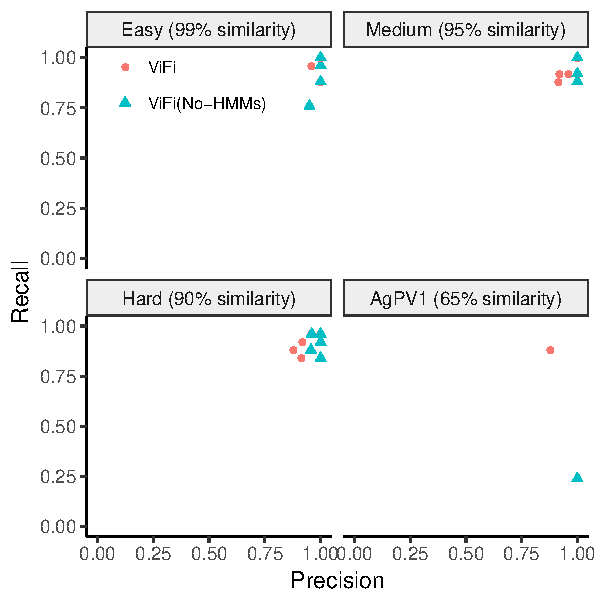
\includegraphics[width=4in]{{results/simulation.all.1000}.pdf}\\
\caption[Results on simulated datasets with 1000 integrations.]
{\label{sim_results_1000}  {\bf Results on simulated datasets.}  We report the recall and precision for four different model conditions with 1000 simulated viral integrations.  We show results for when we include the usage of the  ensemble of HMMs in detecting viral reads (ViFi) and when we exclude the usage of the ensemble of HMMs (ViFi-NoHMMs).  The first three model conditions (easy, medium, and hard) vary the percent similarity of simulated HPV16 genomes to the reference HPV16 genome, with five replicates per simulation.  The last model condition uses Alouatta guariba papillomavirus 1 (AgPV1), a PV genome not included in the set of viral genomes to simulate detection of a novel HPV virus.  AgPV1 is 44\% similar to HPV16.  VERSE failed to complete on any datasets.  All datasets were simulated with 25x coverage.}
\end{figure}



\begin{figure}[htpb]
  \centering
  %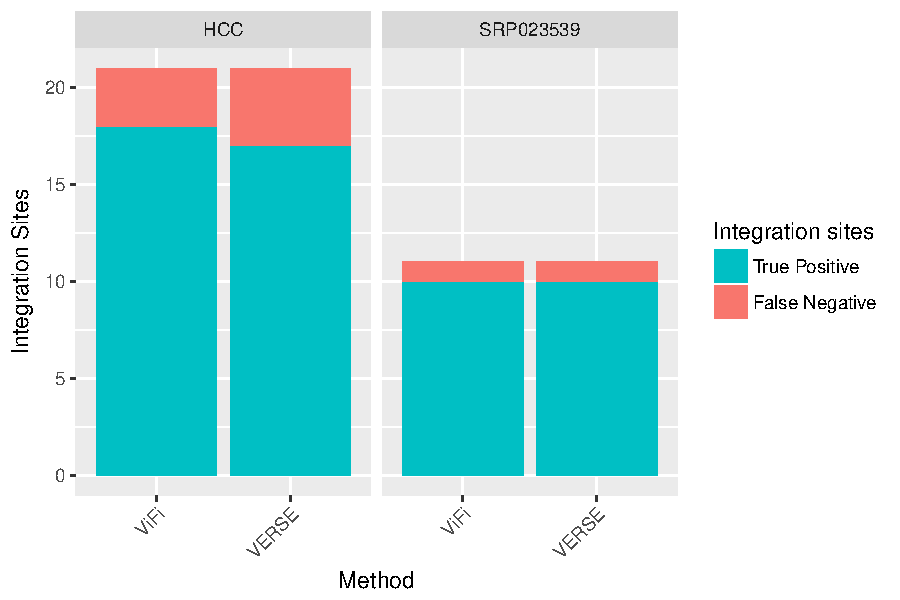
\includegraphics[width=1\linewidth]{results/hcc.pdf}\\
\caption[Recovery of experimentally verified integration sites from biological datasets.]
{\label{bio_results}  {\bf Recovery of experimentally verified integration sites.}  We report the number of experimentally verified integration sites recovered from biological datasets for our method and VERSE.  The datasets include the HCC WGS dataset from the Sung et al. 2012 study (21 experimentally validated integration sites) and the HCC RNAseq cell line dataset from the Lau et al. 2014 study (11 experimentally validated integration sites).}
\end{figure}

%\begin{figure}[htpb]
%  \centering
%  \includegraphics[width=6in]{results/{expected.all.counts.hu.violin}.pdf}\\
%  \caption[Total number of integrations proximal to functional annotation.]  {\label{integration_counts} \textbf{Total number of integrations that are within 25 bps of an annotated type.}  The points give the total number of integrations (e.g. SINE/Alu) within 25 bps of the specific functional annotations in the TCGA-CESC data.  Blue represents results from WGS data, and red represents results from RNA-seq data.  The violin plot shows the distribution of observed breakpoints within 25 bps of the specific annotations across 1,000 replicates, where each replicate is a collection of 226 randomly chosen breakpoints.  The annotated types of interest were taken from the Hu et al. (2015) study~\cite{Hu2015}.   The p-values of the
%  observed number of integrations (Z-test) are all statistically
%  significant for the RNA-seq data(p-value $<10^{-20}$).  The p-values for the WGS data were significant for satellites (p-value $<10^{-20}$), short tandem repeats (p-value $<10^{-16}$), and SINE/Alu (p-value $<0.01$), but not for LTR/ERV1.}
%\end{figure}

%\begin{figure}[htpb]
%  \centering
%  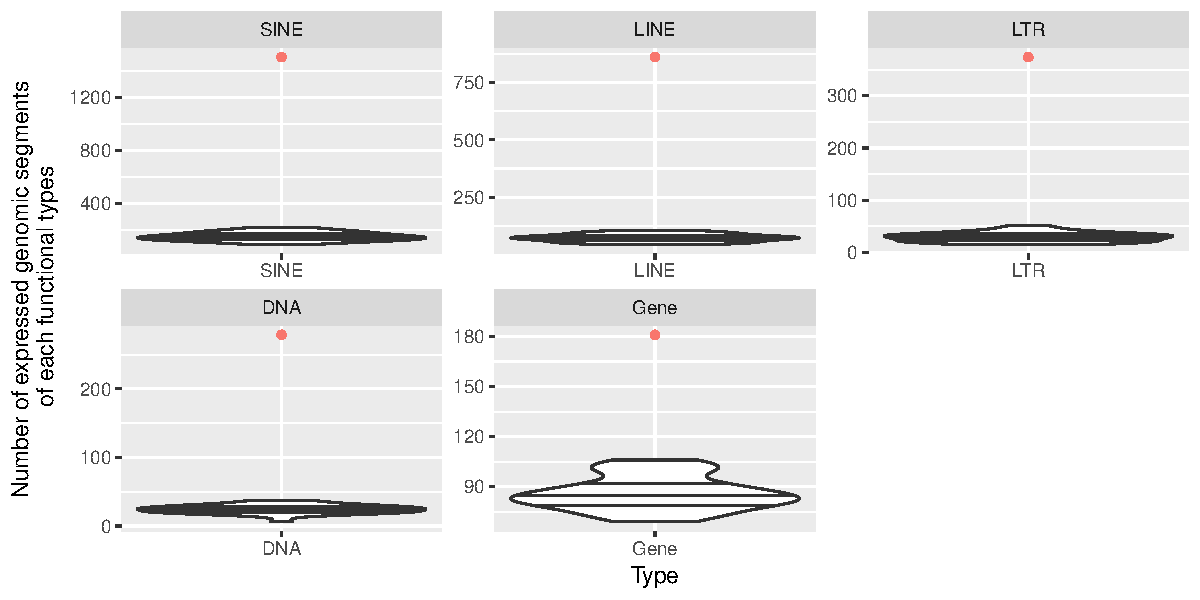
\includegraphics[width=1\linewidth]{{results/expected.wgs.counts.violin}.pdf}\\
%\caption[Annotations of integrated regions.]
%{\label{integration_counts}  {\bf Observed and expected number of annotations of the integrated regions.}  We show the violin plots of the expected number of counts from random integrations for each annotation over 100 simulated experiments, and the actual number of annotations for the observed integrations found in our TCGA-CESC dataset (in red).  The quantiles of the violin plots are displayed with lines.  The p-values of the observed annotation counts (Z-test) are: SINE $<$ 1e-7; LINE $<$ 0.585;	LTR $<$ 0.468;  DNA $<$ 0.56; Gene $<$ 1e-6; and	Oncogenes $<$ 0.179.}
%\end{figure}

%\begin{figure}[htpb]
% \centering
% \includegraphics[width=1\linewidth]{results/{expected.all.total_counts.violin}.pdf}\\
%\caption[Annotations of gene and all repeat elements for transcripts covering the regions containing integrations.]
%{\label{all_classes_count}  {\bf Number of annotated types 
%  covered by WGS or RNA-seq reads across all genomic intervals containing integrations.}  The points give the
%  number of specific functional annotations (e.g. SINE)
%  across all 226 genomic integration sites in the TCGA-CESC data
%  set that are partially covered by at least three reads.  Blue represents results from WGS data, and red represents results from RNA-seq data.  The violin plot show the distribution of the total number of
%  specific annotations across 1,000 replicates that are partially covered by at least three reads, 
%  where each replicate is a collection of 226 randomly chosen intervals.}
%\end{figure}

\begin{figure}[htpb]
 \centering
 %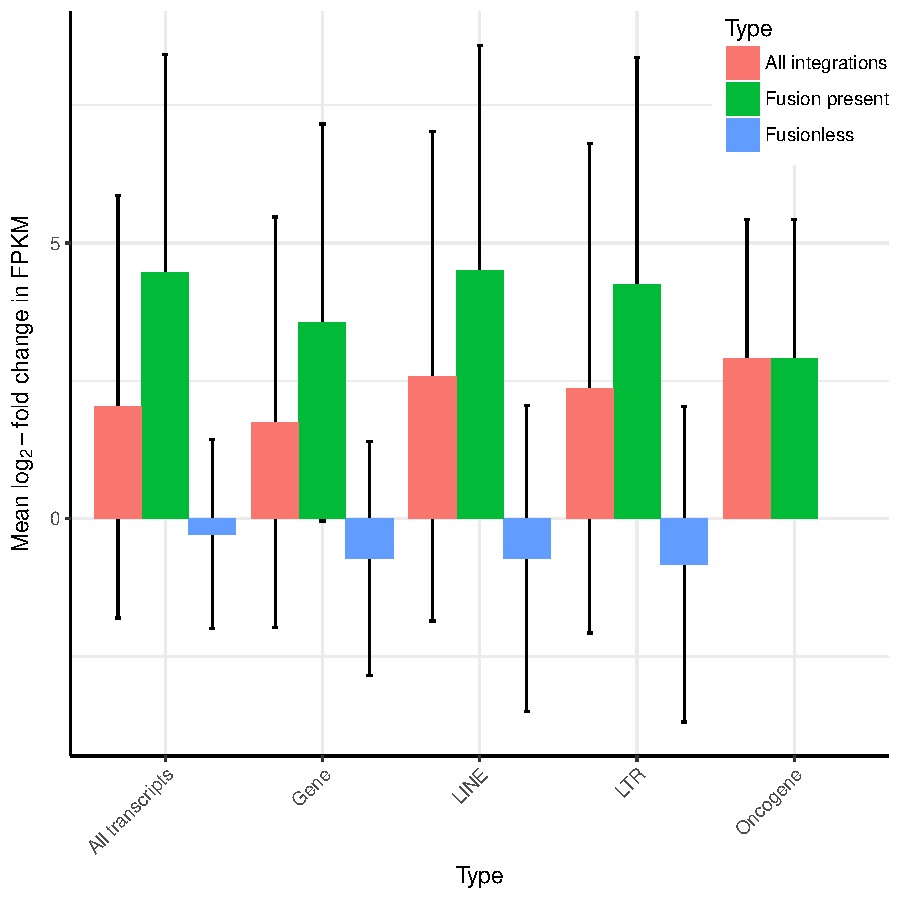
\includegraphics[ width=1\linewidth]{{results/expression.summary.barplot.fold}.pdf}\\
\caption[Expression of mRNA transcripts in genomic segments with and without integrations.]
{\label{expression_transcripts_type}  {\bf Log2 fold change in expression of mRNA transcripts in genomic segments with and without integrations.}  We report the Log2 fold change in expression of annotated features between genomic segments with and without integrations.  We report the average fold change for all segments, segments that contain fusion mRNA sequences, and segments without fusion mRNA sequences.  For a given integration in a sample, we select a 10kb flanking region around the integration site.  We then report the logfold change in expression level in samples that have an integration in this region and samples that do not.}
\end{figure}

\begin{figure}[htpb]
  \centering
  %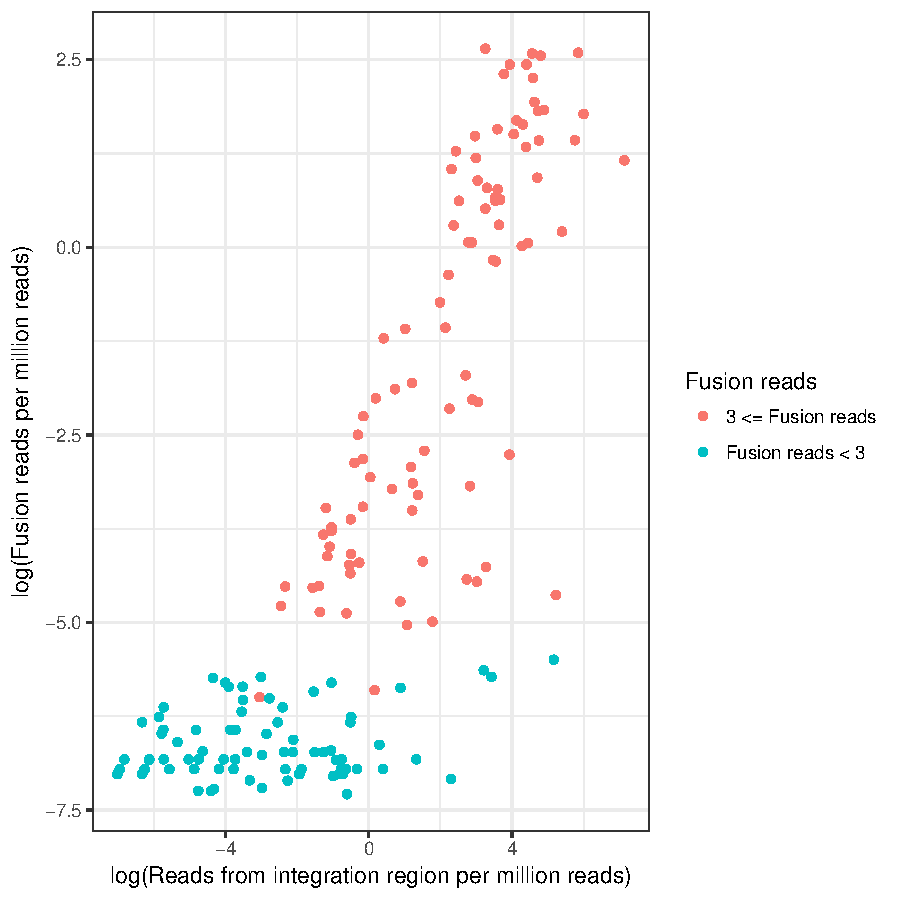
\includegraphics[ width=1\linewidth]{{results/chimierc.log}.pdf}\\
\caption[Correlation between number fusion mRNA reads per million to total mRNA reads per million.]  {\label{corr_plot} {\bf Correlation between proportion of fusion mRNA reads to total mRNA reads within an integration region.}  For each genomic interval, we report the log$\_10$ of the total number of fusion mRNA reads per million reads for an integration region compared to the log$\_10$ of the total number of mRNA reads per million reads within the same integration region.  Red points have three or more fusion reads present in the interval; blue points have fewer than three fusion reads.}
\end{figure}

\begin{figure}[htpb]
  \centering
  %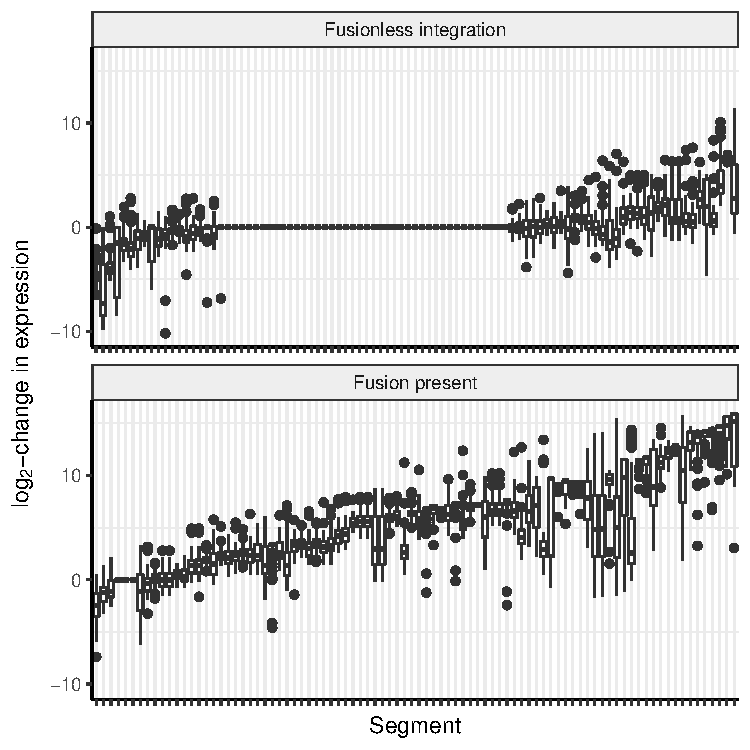
\includegraphics[ width=1\linewidth]{{results/wgs.fpkm.all.boxplot.10000}.pdf}\\
\caption[Log$_2$-fold change of expression between genomic segments with
  and without integrations.]  {\label{all_expression_box} {\bf Boxplots of
    log-fold change of expression between genomic segments with and
    without integrations.}  We show boxplots of the Log$_2$-fold change
  in expression of genomic regions with and without integrations.  The
  genomic regions are separated by whether or not there are associated
  fusion transcriptions within the interval containing the genomic integration.}
\end{figure}

\begin{figure}[htpb]
  \centering
  %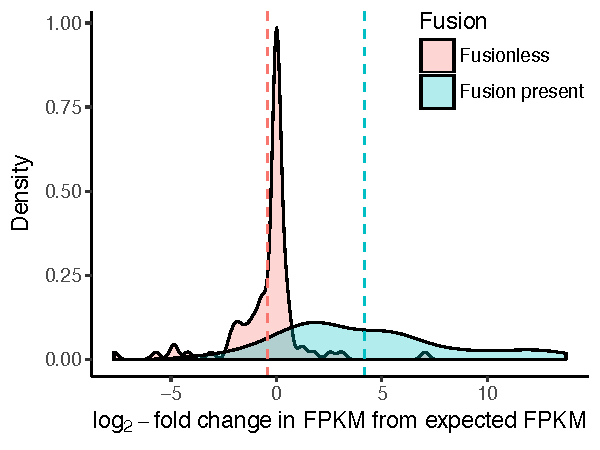
\includegraphics[ width=1\linewidth]{{results/cnv_fold_change}.pdf}\\
\caption[The distribution of log$_2$-fold change in expression of human mRNA between segments with and without integrations, normalized for copy number variation.]  {\label{cnv_fold_change} {\bf The distribution of log$_2$-fold change in expression of human mRNA between segments with and without integrations, normalized for copy number variation.}  For a particular genomic region, we compute the mean expected FPKM per copy number by taking the mean of the total FPKM divided by the average copy number of the region for each sample not containing the integration.  We compute the expected fold change as the FPKM of the genomic region divided by the average copy number of that region for the sample containing the integration divided by the mean expected FPKM per copy number.  The dashed lines show the average log-fold change.}
\end{figure}


%\begin{figure}[htpb]
% \centering
% 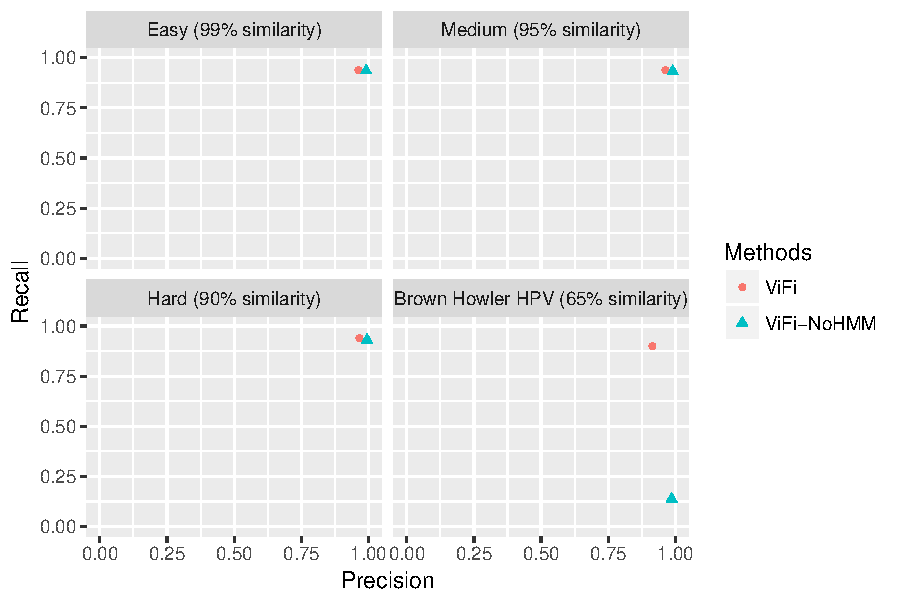
\includegraphics[width=1\linewidth]{{results/simulation.1000}.pdf}\\
% \caption[Precision-recall on simulated datasets with 1000 viral integrations.] {{\bf Precision-recall on simulated datasets.  \label{sim_results_1000}}  We report the recall and precision for four different model conditions.  We show results for when we include the usage of the  ensemble of HMMs in detecting viral reads (Default) and when we exclude the usage of the ensemble of HMMs (Default-NoHMMs).  The first three model conditions (easy, medium, and hard) vary the percent similarity of simulated HPV16 genomes to the reference HPV16 genome, with five replicates per simulation.  The last model condition uses Alouatta guariba papillomavirus 1 (AgPV1), an HPV genome not included in the set of viral genomes to simulate detection of a novel HPV virus.  AgPV1 is 44\% similar to HPV16.  VERSE failed complete on any datasets.  All datasets were simulated with 25x coverage.}
%\end{figure}

%\begin{figure}[htpb]
% \centering
% 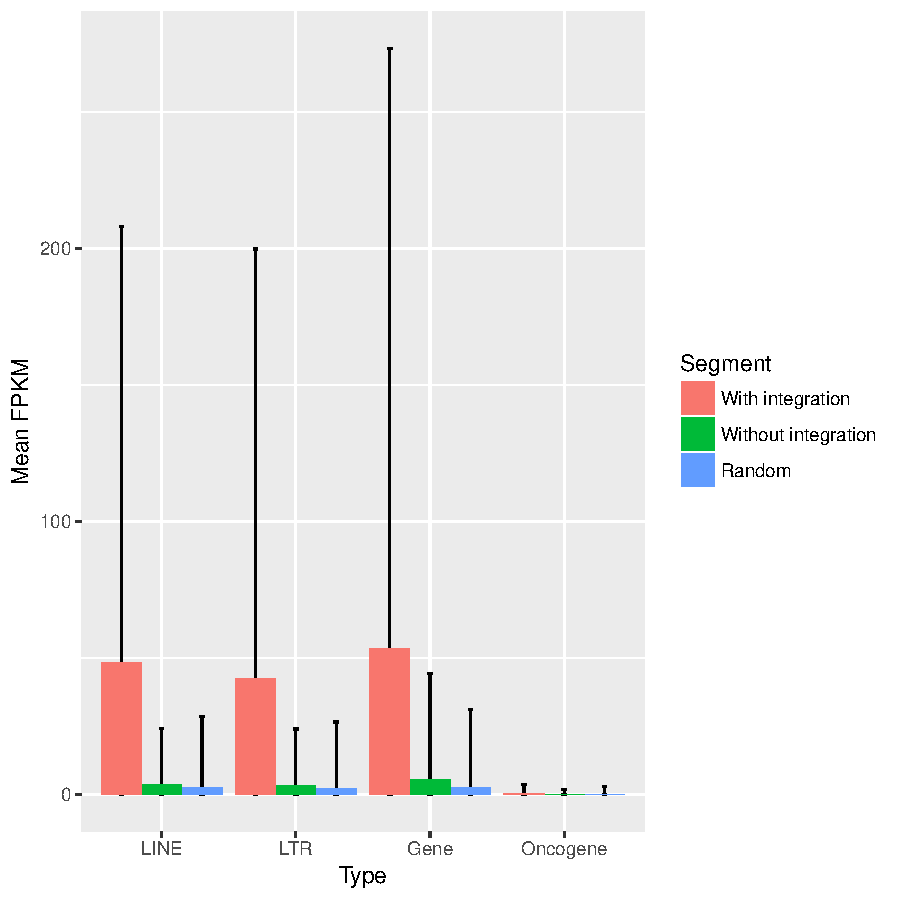
\includegraphics[width=1\linewidth]{{results/expression.summary.barplot}.pdf}\\
%\caption[Expression of mRNA transcripts in genomic segments with and without integrations.]
%{\label{expression_transcripts_fpkm}  {\bf Expression of mRNA transcripts in genomic segments with and without integrations.}  We report the mean FPKM expression of annotated features in genomic segments with and without integrations.  For a given integration in a sample, we select a 10kb flanking region around the integration site.  We then report the expression level in samples that have an integration in this region and samples that do not.  In addition, we report the expression level randomly selected segments as a baseline. The p-values for the paired Wilcoxon signed rank test of the difference in FPKM expression for genomic segments with and mean FPKM expression in segments without integrations are: LINE $<$ 1e-12;	LTR < 1e-10;  Gene < 1e-10; and	Oncogenes < NA.}
%\end{figure}

\begin{figure}[htpb]
  \centering
  %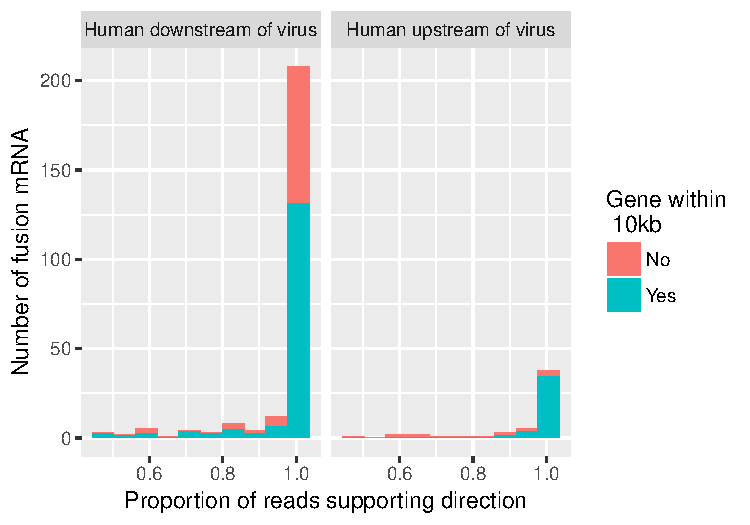
\includegraphics[width=1\linewidth]{{results/rna_direction.summary.histogram}.pdf}\\
\caption[Orientation of the mRNA fusion transcripts.]
{\label{mrna_directions}  {\bf Orientation of the mRNA fusion transcripts.}  We report whether the human portion of the fusion mRNA sequences are upstream or downstream of the viral portion.  The orientation is inferred from the paired-end reads under the assumption that the viral read is always oriented in the direction of the viral gene, and support for the orientation is computed as the proportion of paired-end reads supporting that orientation.  In addition, we report whether there is a gene within 10kb of the fusion mRNA read.}
\end{figure}

\begin{figure}[htpb] \centering
  %\includegraphics[width=4in]{{classification}.pdf}\\
  \caption[Classification of integrations.]  {\label{classification} {\small {\bf
        Classification of integration types using fusion mRNA.}  We classify integrations as
        `simple', `complex', and `fusionless'.  An integration is denoted as
      `fusionless' when it does not contain a mapped chimeric
      (viral-human mRNA); otherwise, it is denoted as `simple' when it
      is the only integration within a 10kb window, and at least 75\%
      of the chimeric paired-end reads supporting a fusion mRNA event
      are oriented in the same direction relative to the viral
      gene. All other regions are denoted `complex'}} %35,
\end{figure}



\begin{figure}[htpb]
  \centering
  %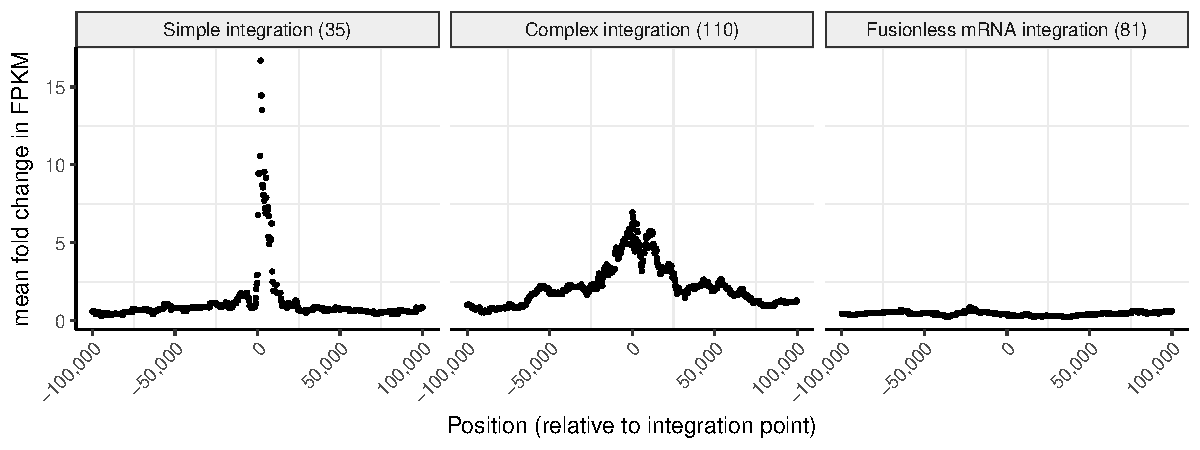
\includegraphics[width= 4in]{{results/updown.100000}.pdf}
\caption[Fusion reads supp.]
{\label{updown_100kb}  {\bf Expression change around integration point within a 100kb window}.  We report the average fold expression change upstream and downstream of an integration event within a 100kb window.  The position is reported relative to the integration point in the human genome, with negative position being upstream of the integration event, and positive position being downstream of the integration event.  The results are separated out by the integration category. } %35, 110, 81
\end{figure}

\begin{figure}[htpb]
  \centering
  %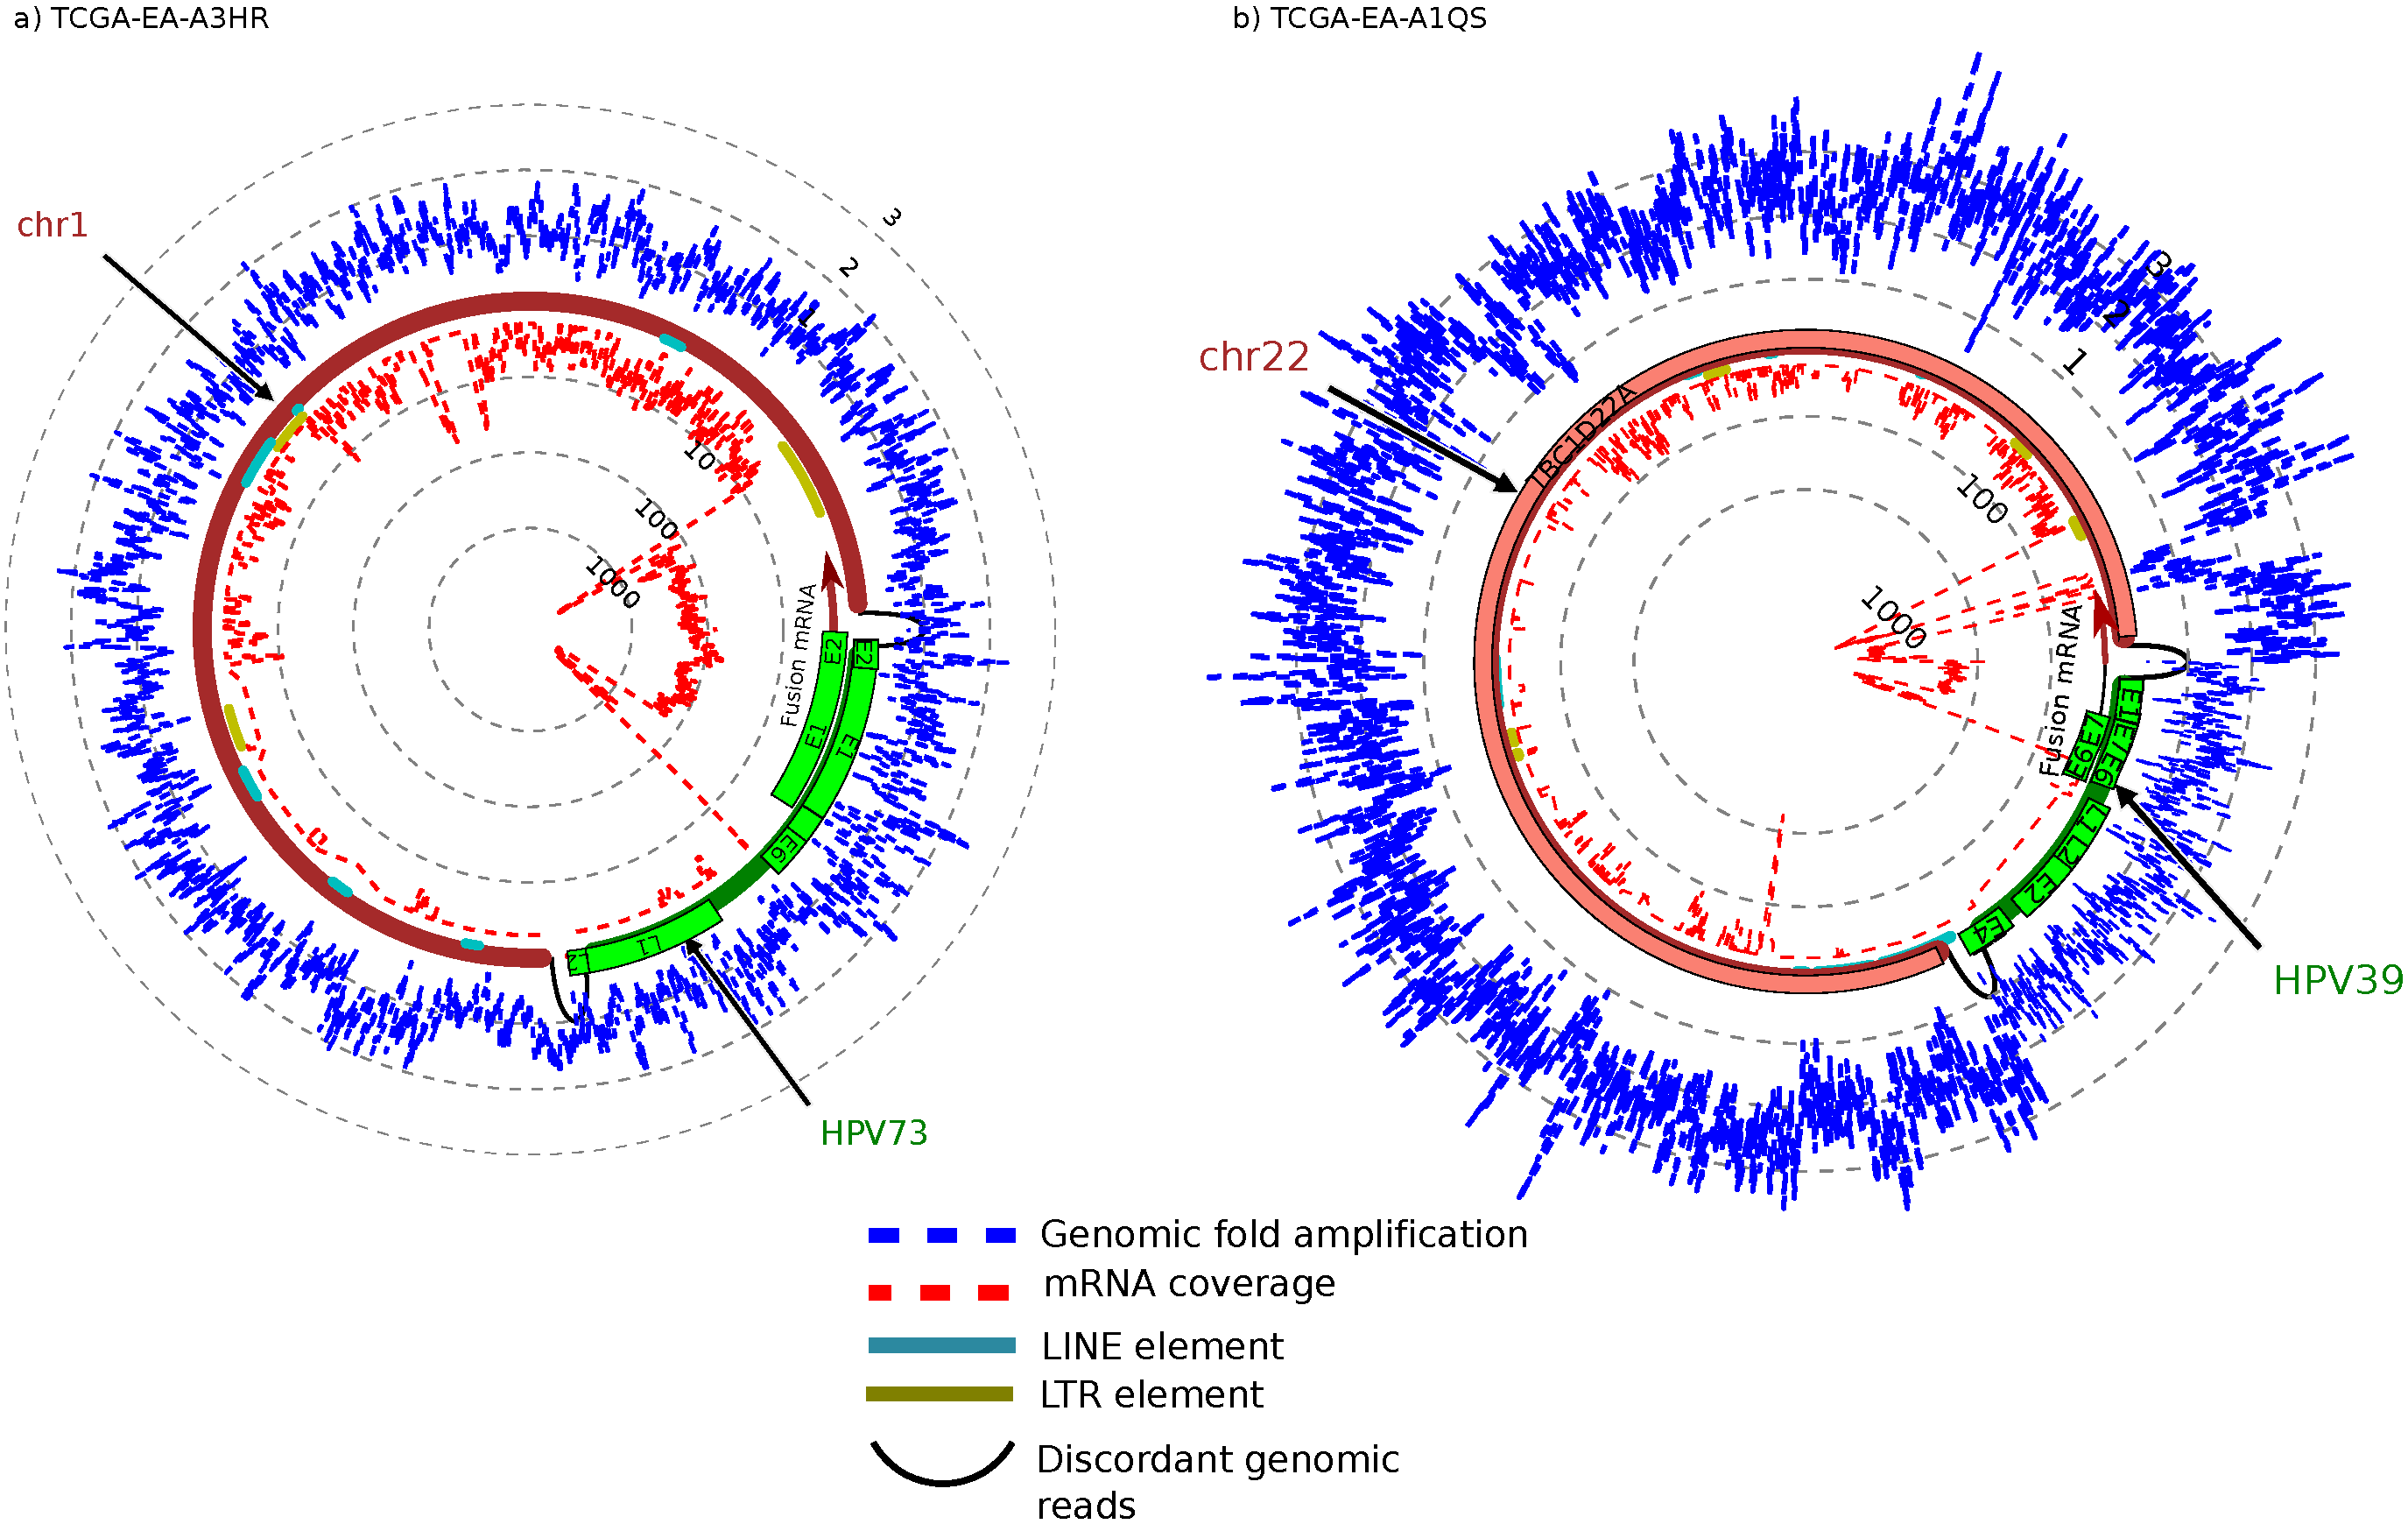
\includegraphics[width=6.5in]{{results/combined_ecdna}.pdf}
%  \subfloat[TCGA-C5-A0TN.]{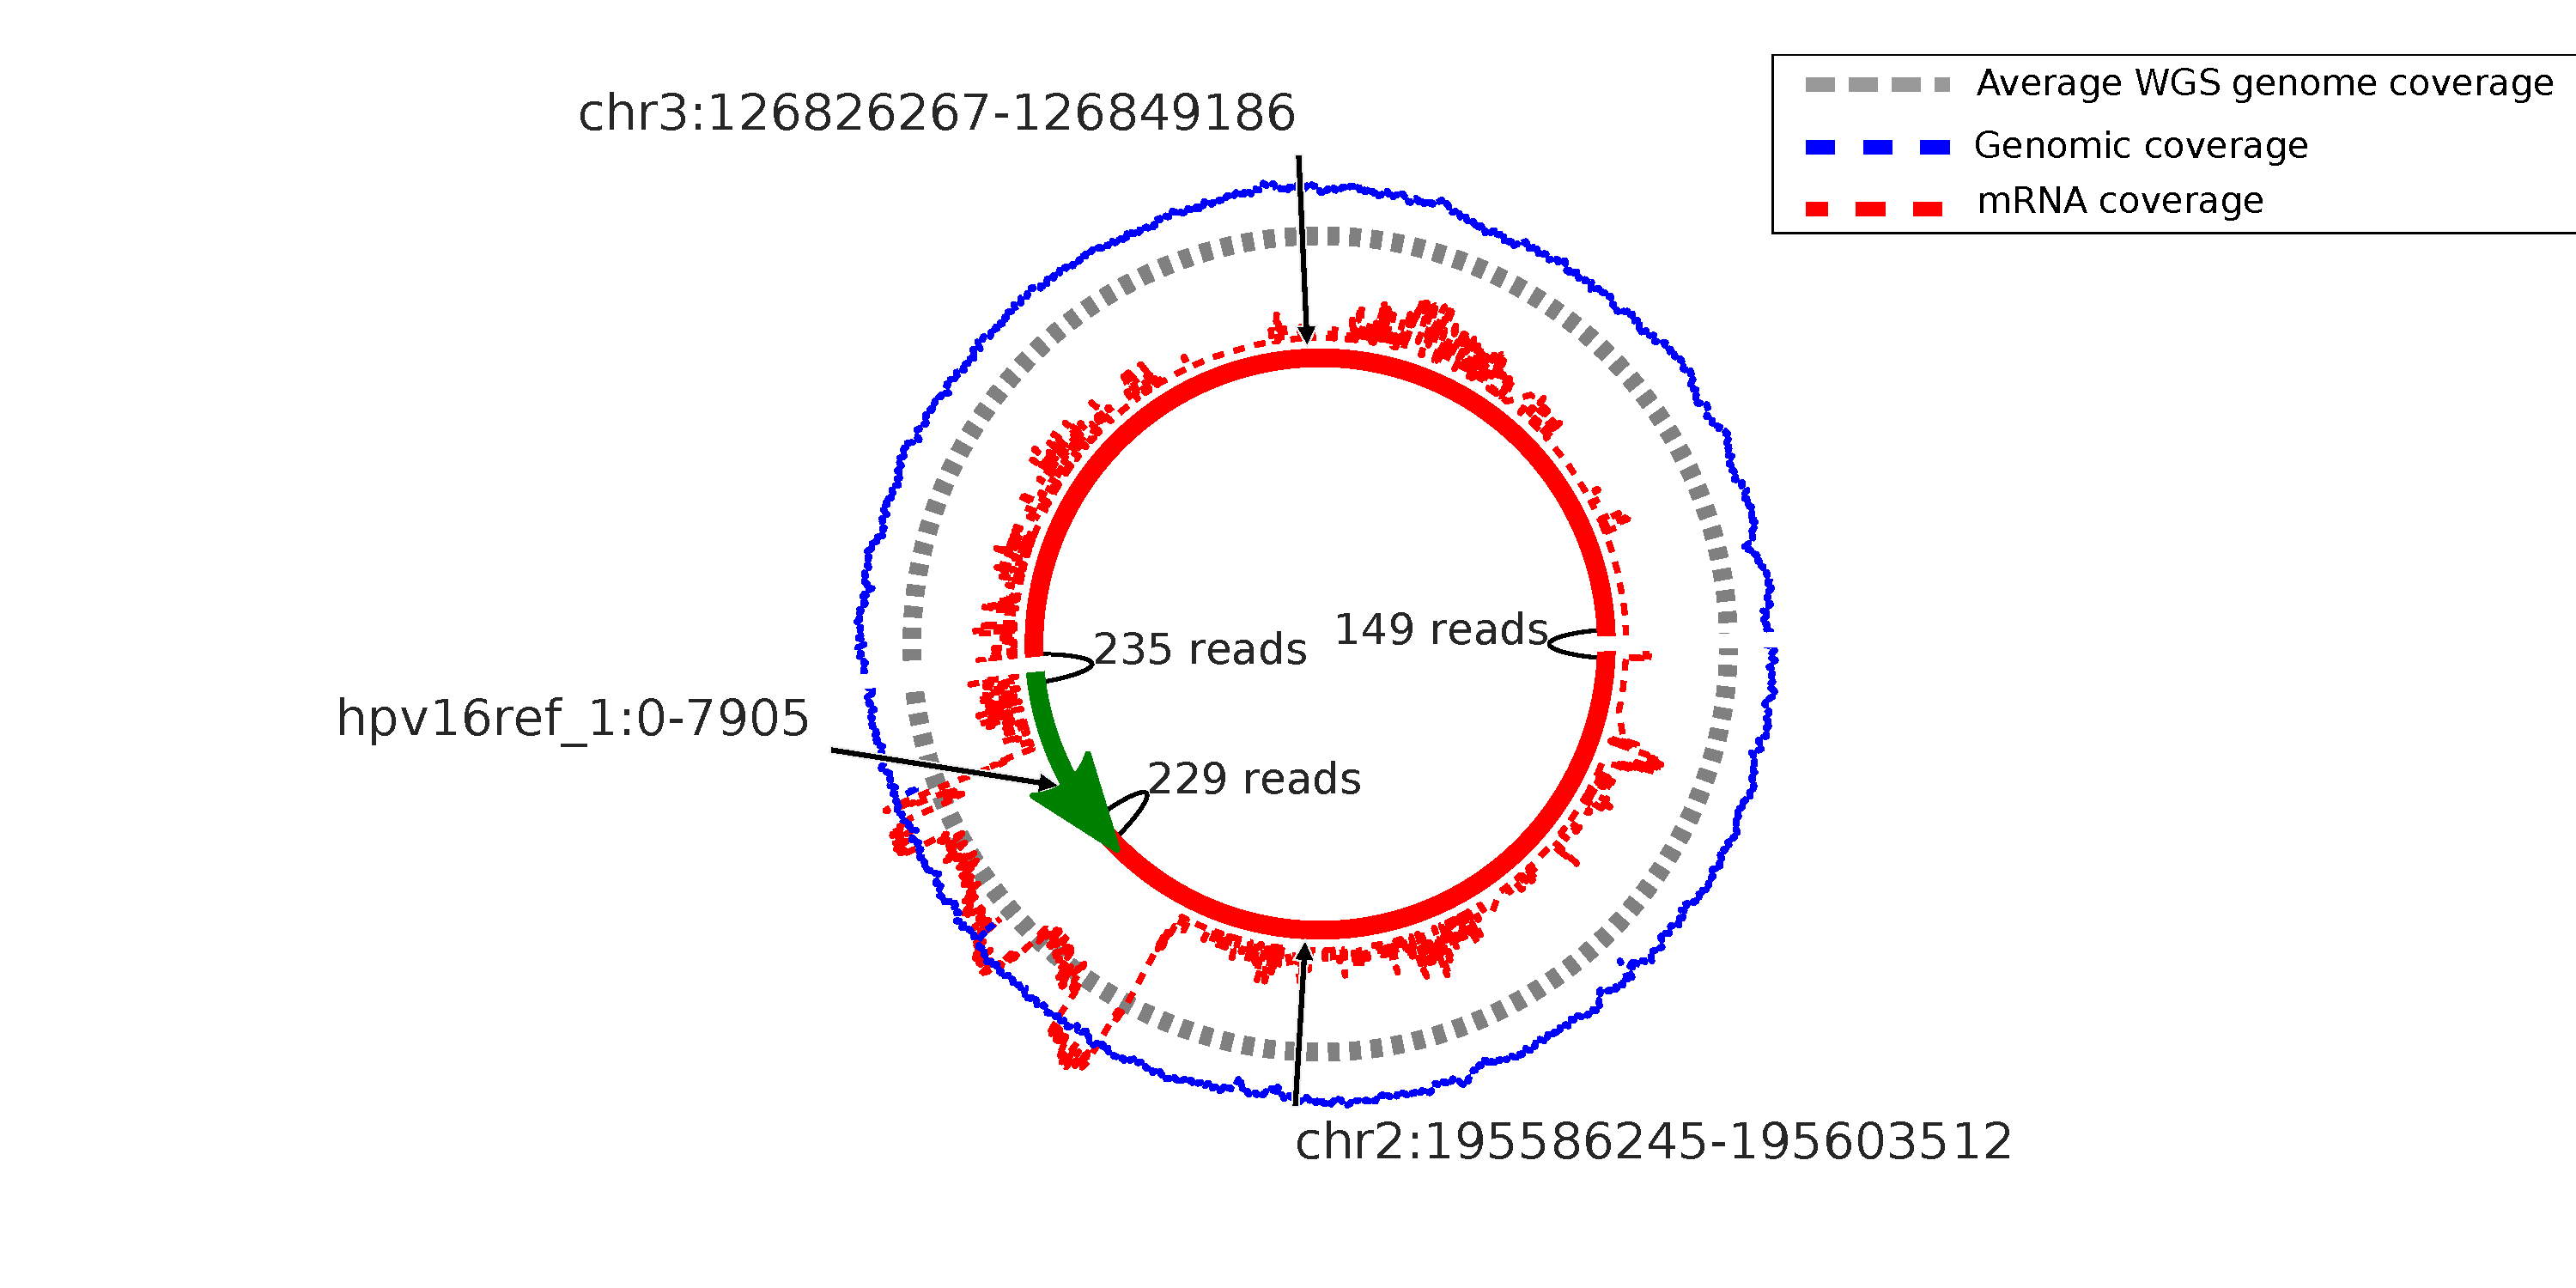
\includegraphics[width=3in,frame]{{results/TCGA-C5-A0TN.annotated}.pdf}}
%  \subfloat[TCGA-EK-A2RE.]{\includegraphics[width=6in]{{results/TCGA-EK-A2RE-annotated}.pdf}}\\  
%  \subfloat[TCGA-EA-A1QS.]{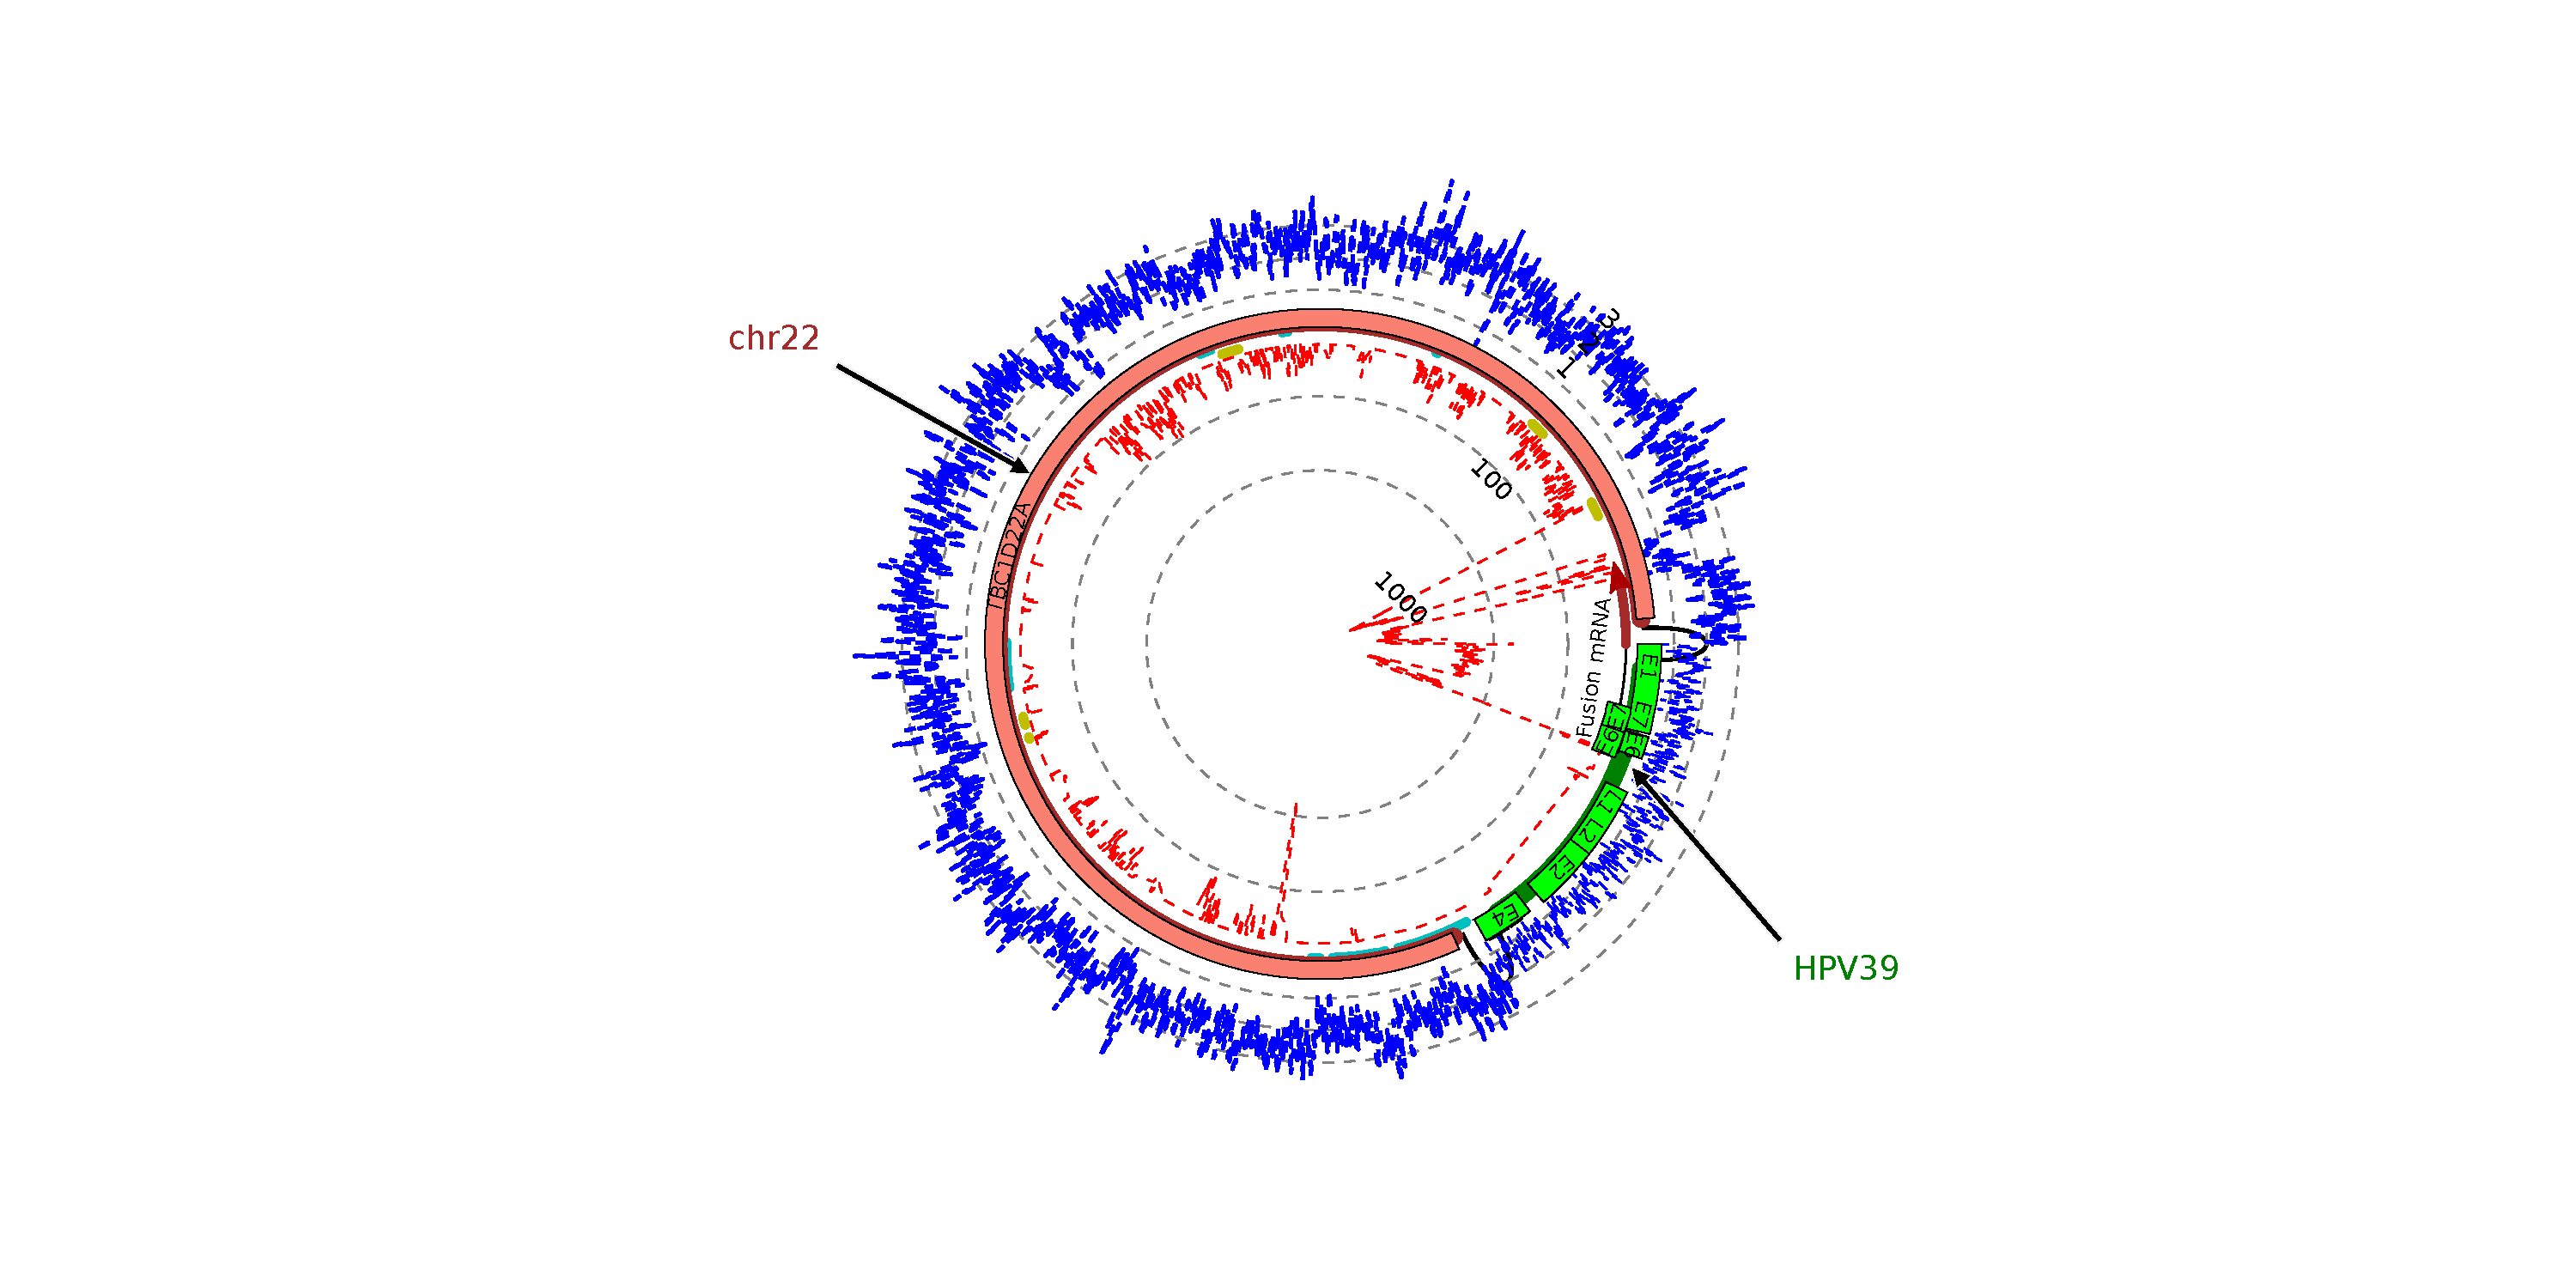
\includegraphics[width=6in]{{results/TCGA-EA-A1QS-annotated}.pdf}}\\
%  \subfloat[TCGA-EA-A3HR.]{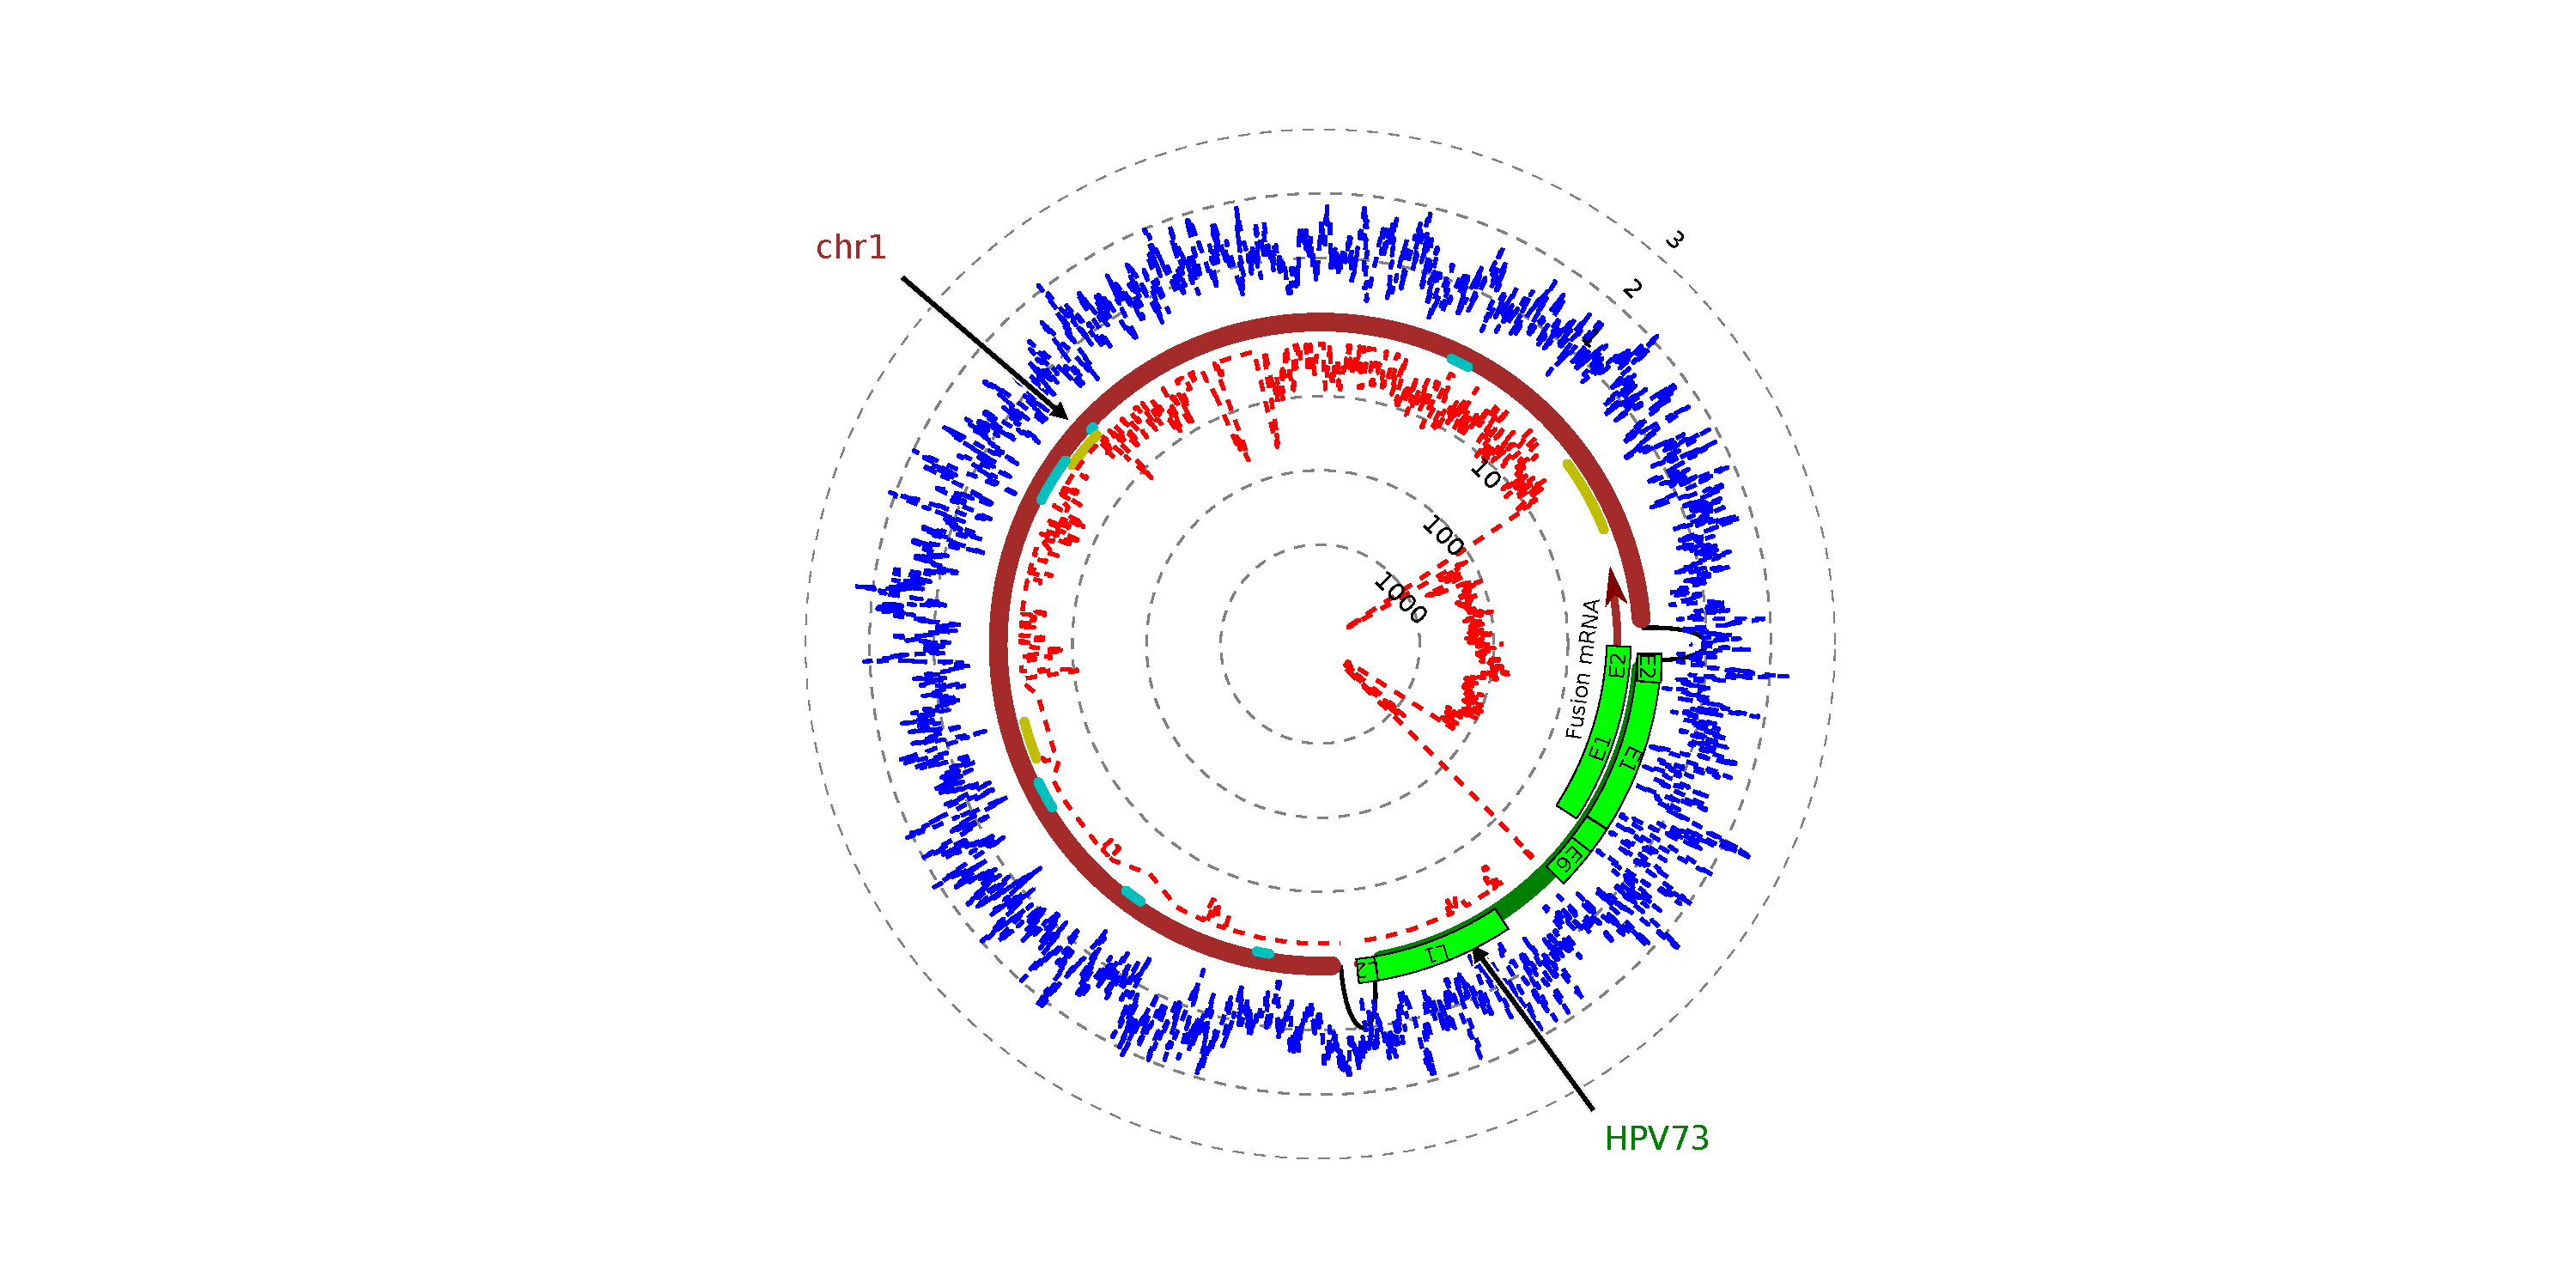
\includegraphics[width=6in]{{results/TCGA-EA-A3HR-annotated}.pdf}}\\    
\caption[Proposed ecDNA structures.]
{\label{ecDNA_supp}  {\bf Proposed ecDNA structures.}  Proposed ecDNA structure for integrations from a) TCGA-EA-A3HR and b) TCGA-EA-A1QS.  The genomic coverage fold amplification of the region relative to the average genomic coverage of the entire genome is shown in blue, and the mRNA coverage of the region is shown red.  LINE and LTR elements are highlighted in teal and gold, respectively.  The viral genes are highlighted in light green, and human genes are highlighted in light red.  The assembled fusion transcript from this region is shown in the figures.  }
\end{figure}
\clearpage
\bibliographystyle{naturemag}
\def\bibfont{\normalsize}
\bibliography{main}
\end{document}
